\section{Hardware}
\label{sec:hardware}

This system required a significant amount of additional hardware. The most
important part of the off-chip circuitry was the flex sensors used to detect
player grabbing. When the player grabs in reality, the flex sensor is bent, and
its resistance changes. The flex sensor is placed in series with another
resistor to create a variable voltage divider. A second voltage divider,
comprising simply of two resistors, creates a threshold voltage. Both of these
are then used as inputs to an op amp, which acts as a comparator, outputting a 0
or 5 volt signal to the fpga. While simple in design, the flex sensors were much
more difficult to work with in practice. As the game was tested and the sensors
endured strain, they became permanently bent, reducing their change in
resistance. Additionally, they did not have a proportionally large resistance
change to begin with (at best ranging from ~50 to 80 kOhms). This increasingly
lessening change in resistance, combined with their tendency to drift over time,
led to them being less than ideal for the project. A much simpler and reliable
alternative would have been simply including a button on the players palm to
indicate grabbing. Another alternative to be considered for future designs is
using two metal contacts on the players fingertips and palms. One helpful design
choice that made the current implementation possible was to use a potentiometer
instead of a normal resistor in the threshold voltage divider. This allowed a
much quicker, and more precise setting of the threshold voltage. This proved to
be extremely helpful if any of the resistances drifted. Although not ideal, the
flex sensors worked well enough for the project. Additionally, due to lab kit
malfunctions, the circuitry was switched onto a new labkit at the last minute,
which may have caused additional grabbing issues.

The second main piece of hardware used was the vibrating motors. Although small,
they provided a strong force. However, when they vibrated, they drastically
lowered the power supply voltage on the fpga, having a large negative effect on
the grab detection. Because the motors were used to indicate when a player was
able to grab a hold, the haptic feedback was chosen to be removed from the final
version of the project. A photo of the gloves, and off-chip circuitry can be
seen in figures \ref{fig:hardware}

\begin{figure}[h]
\centering
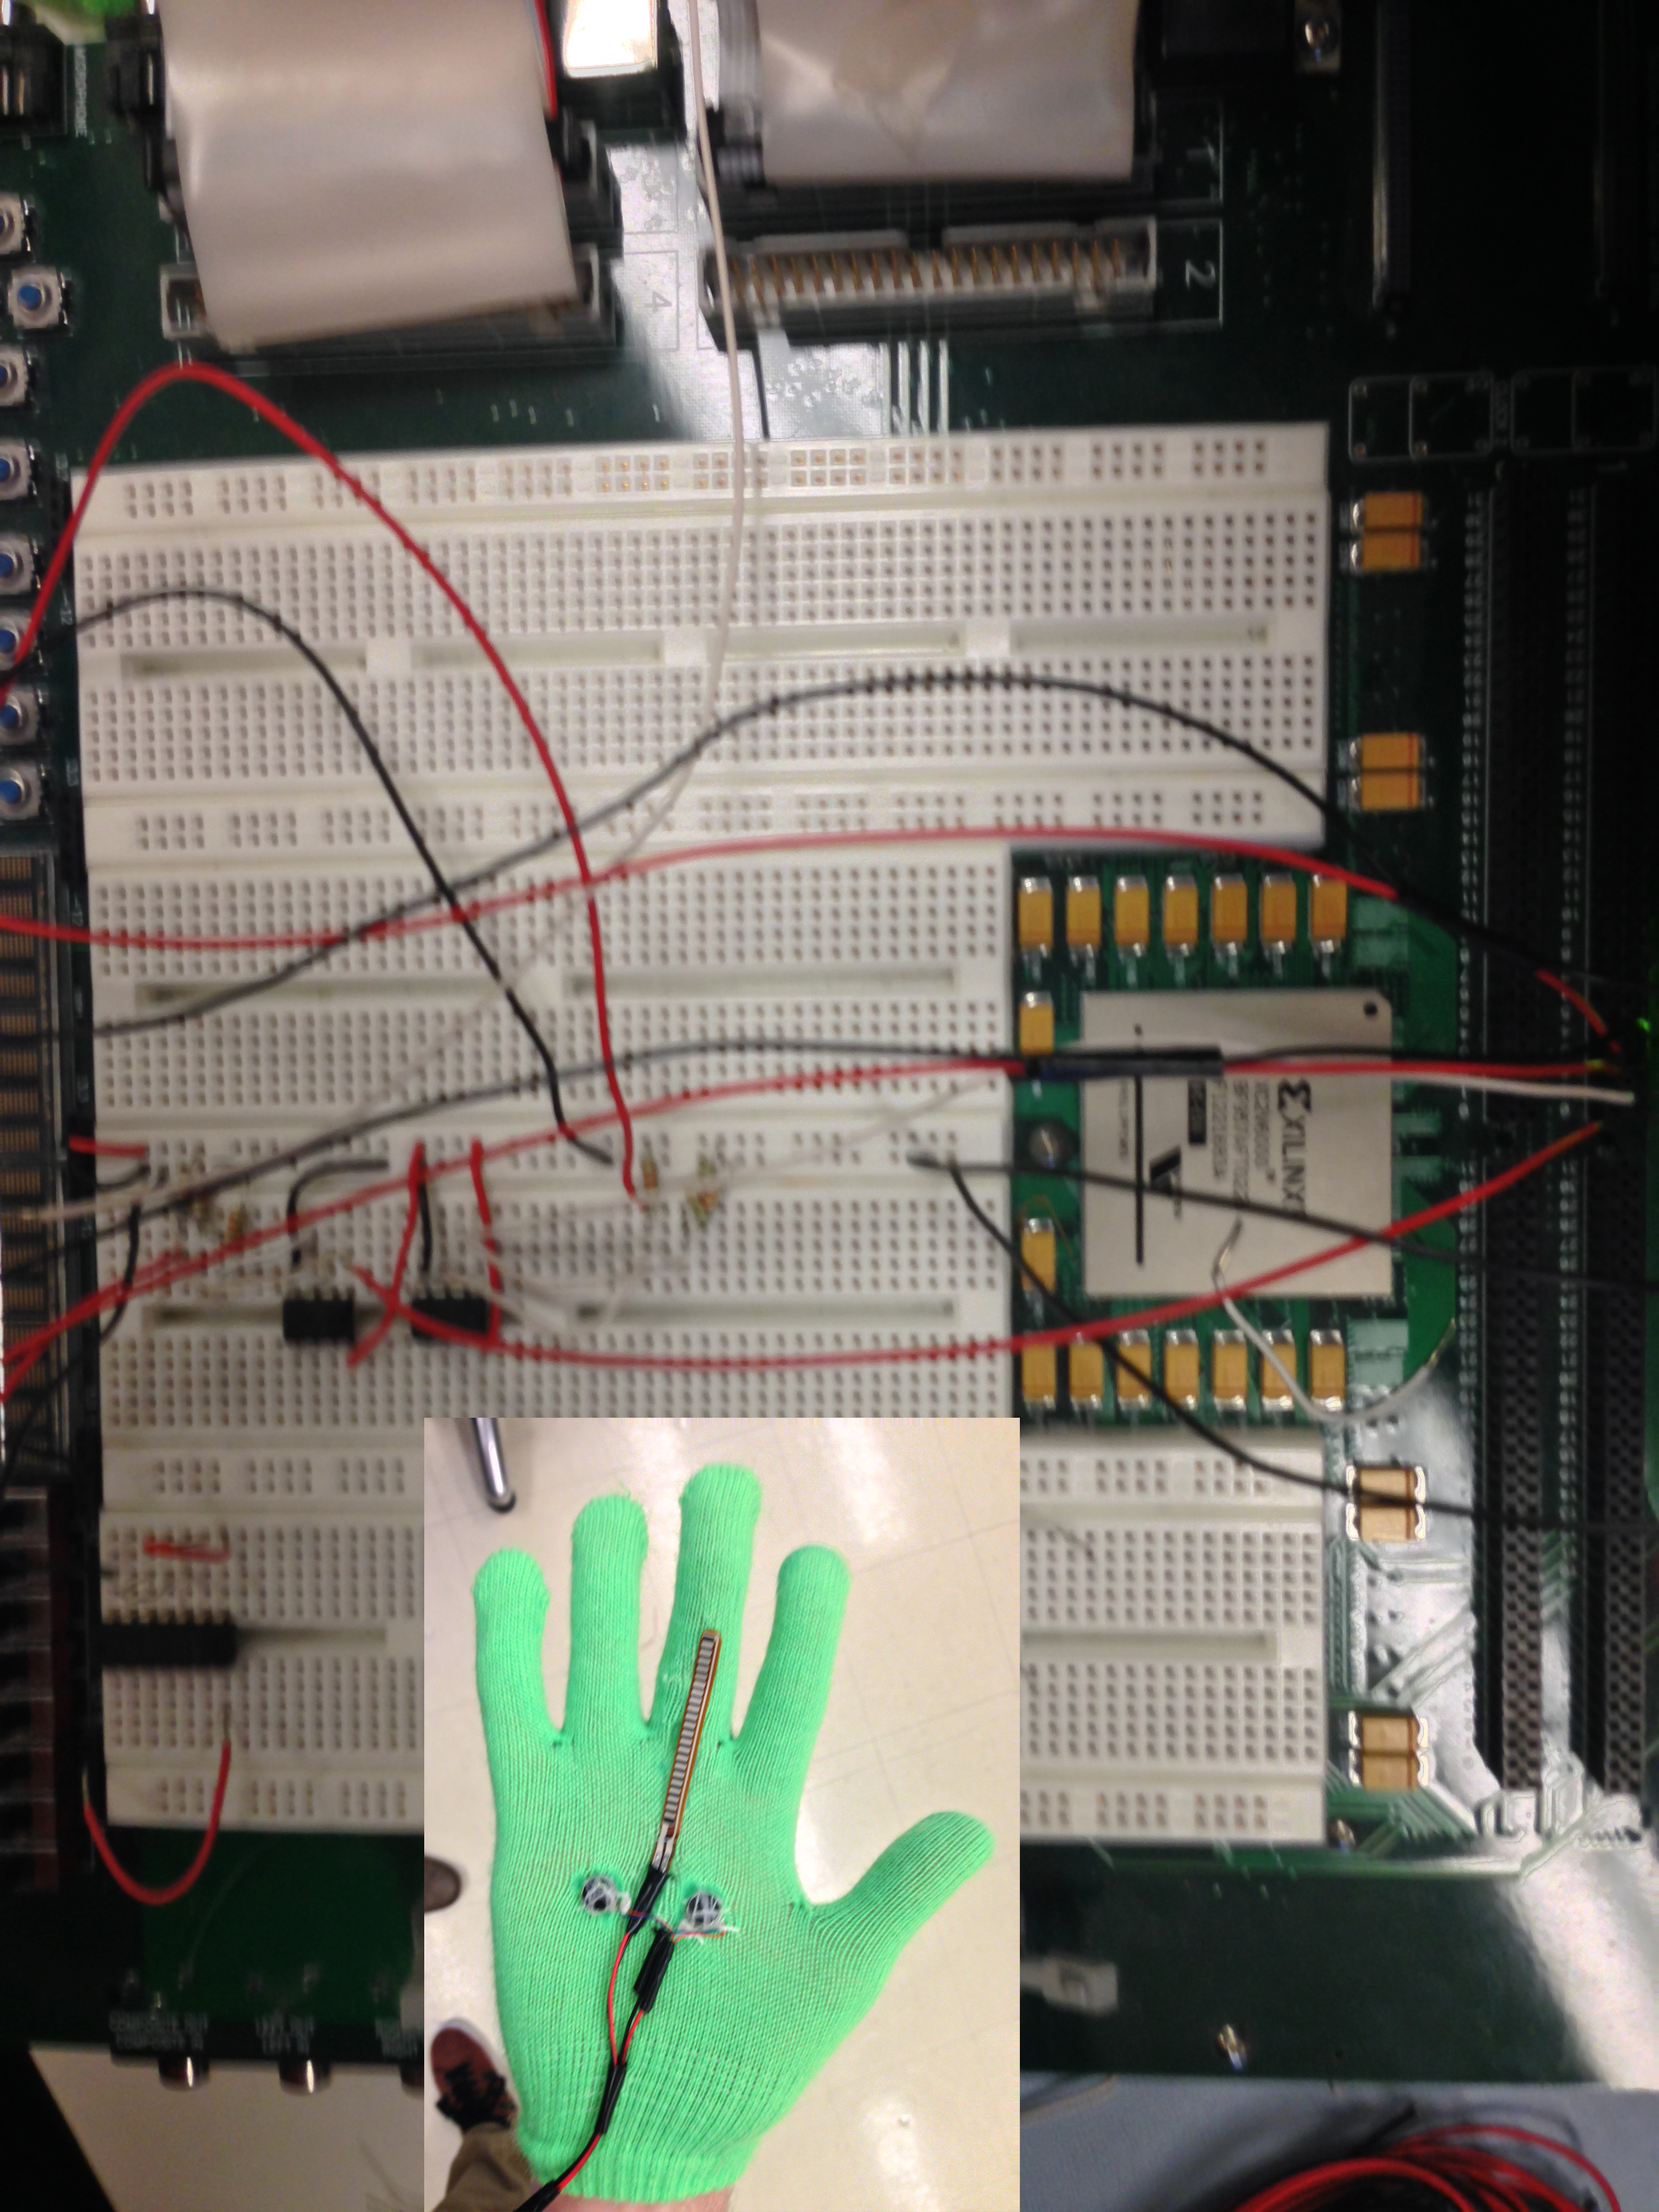
\includegraphics[width=6.5in]{img/hardware.png}
\caption{Apair of circuits built on to the lab kit convert the variable
resistance of the flex sensors into a digital signal. This is done by comparing
the voltage of two voltage dividers, one using set resistor values, and one
using on set value and a flex sensor as the second resistor. The glove itself
has the flex sensor and two motors attached directly to it.}
\label{fig:hardware}
\end{figure}
